%%-----------------------------------------------------------------------%%
%%--- Trees and Forests -------------------------------------------------%%

\chapter{Trees and Forests}
\label{chap:trees_forests}

Recall, a path in a graph $G=(V,E)$ whose start and end vertices are the same is
called a cycle. We say $G$ is {\it acyclic}, or a {\it forest}, if it
has no cycles.
A vertex of a forest of degree one is called an {\it endpoint} or a {\it leaf}.
\index{acyclic}
\index{forest}
\index{endpoint}
\index{leaf}
A connected forest is a {\it tree}.
\index{tree}

A {\it rooted tree} is a tree with a specified {\it root} vertex $v_0$. (However,
if $G$ is a rooted tree with root vertex $v_0$ and if the degree of
$v_0$ is one then, by convention, we do not call $v_0$ an endpoint or
a leaf.)
\index{tree!rooted}
A {\it directed tree} is a directed graph which would be a tree if the
directions on the edges were ignored.
\index{tree!directed}
A rooted tree can be regarded as a directed tree since you image an
edge $E=\{u,v\}$, for $u,v\in V$, being directed from $u$ to $v$,
$e=(u,v)$, if and only if $v$ is further away from $v_0$ that $u$ is.
If $e=(u,v)$ is an edge in a rooted tree then we call $v$
a {\it child} vertex with {\it parent} $u$.
An {\it ordered tree} is a rooted tree for which an ordering is specified
for the children of each vertex.
\index{tree!ordered}
\index{parent}
\index{child}
An {\it $n$-ary tree} is a rooted tree for which each vertex
which is not a leaf has at most $n$ children. The case $n=2$
are called {\it binary trees}.
\index{tree!binary}
\index{tree!$n$-ary}

Directed trees are pervasive in theoretical computer science, as they are
useful structures for describing algorithms and relationships between
objects in certain data sets.

A {\it spanning tree} $T$ of a connected, undirected graph $G$ is a
subgraph containing all vertices of $G$ which is a tree.


\begin{example}
\label{example:span-tree}
{\rm
Consider the $3\times 3$ grid graph with $16$ vertices and
$18$ edged. Two example of a spanning tree are given in Figure
\ref{fig:span-tree1} by using thicker line width for its edges.


\begin{figure}[h!]
\begin{center}
\begin{tabular}{cc}
% this was done "manually"
\unitlength=0.620000pt
\begin{picture}(210.00,192.00)(0.00,0.00)
%\put(-3.00,-3.00){$\bullet$} % vertices look funny
%\put(-3.00,189.00){$\bullet$}
%\put(61.00,189.00){$\bullet$}

\thinlines
\put(0.00,192.00){\line(1,0){192.00}} %outer box
\put(192.00,0.00){\line(0,1){192.00}} %outer box
\put(0.00,0.00){\line(1,0){192.00}} %outer box
\put(0.00,0.00){\line(0,1){192.00}} %outer box

\put(0.00,64.00){\line(1,0){192.00}} %inner lines
\put(0.00,128.00){\line(1,0){192.00}} %inner lines

\put(64.00,0.00){\line(0,1){192.00}} %inner lines
\put(128.00,0.00){\line(0,1){192.00}} %inner lines

\linethickness{0.9mm}  % tree edges
\put(0.00,0.00){\line(0,1){64.00}}
\put(0.00,0.00){\line(1,0){192.00}}
\put(64.00,0.00){\line(0,1){64.00}}
\put(64.00,64.00){\line(1,0){128.00}}

\put(192.00,64.00){\line(0,1){64.00}}

\put(0.00,128.00){\line(1,0){192.00}}
\put(0.00,128.00){\line(0,1){64.00}}
\put(64.00,128.00){\line(0,1){64.00}}
\put(128.00,128.00){\line(0,1){64.00}}

\put(128.00,192.00){\line(1,0){64.00}}
\end{picture}

&
% this used jPicEdt
\unitlength=2.000000pt
\begin{picture}(80,80)(20,20)
\linethickness{0.3mm}
\put(20,80){\line(1,0){20}}
\linethickness{0.3mm}
\put(40,80){\line(1,0){20}}
\linethickness{0.3mm}
\put(40,60){\line(0,1){20}}
\linethickness{0.3mm}
\put(60,60){\line(0,1){20}}
\linethickness{0.3mm}
\put(20,60){\line(1,0){60}}
\linethickness{0.3mm}
\put(80,60){\line(0,1){20}}
\linethickness{0.3mm}
\put(60,80){\line(1,0){20}}
\linethickness{0.3mm}
\put(20,20){\line(0,1){60}}
\linethickness{0.3mm}
\put(20,20){\line(1,0){60}}
\linethickness{0.3mm}
\put(80,20){\line(0,1){40}}
\linethickness{0.3mm}
\put(60,20){\line(0,1){40}}
\linethickness{0.3mm}
\put(40,20){\line(0,1){40}}
\linethickness{0.3mm}
\put(20,40){\line(1,0){60}}
\linethickness{0.3mm}

\linethickness{0.9mm}
\put(20,80){\line(1,0){60}}
\linethickness{0.9mm}
\put(80,60){\line(0,1){20}}
\linethickness{0.9mm}
\put(20,60){\line(1,0){60}}
\linethickness{0.9mm}
\put(40,40){\line(0,1){20}}
\linethickness{0.9mm}
\put(60,40){\line(0,1){20}}
\linethickness{0.9mm}
\put(20,40){\line(1,0){20}}
\linethickness{0.9mm}
\put(20,20){\line(0,1){20}}
\linethickness{0.9mm}
\put(20,20){\line(1,0){60}}
\linethickness{0.9mm}
\put(80,20){\line(0,1){20}}
\end{picture}
\end{tabular}
\caption{Spanning trees for the $4 \times 4$ grid graph.}
\end{center}
\label{fig:span-tree1}
\end{figure}

}
\end{example}



The following game is a variant of the Shannon switching game, due to
Edmunds and Lehman. We follow the description in Oxley's
survey ({\it What is a matroid?'} ... add reference later ... ).

Recall a minimal edge cut of a graph is also called a bond of the graph.
\index{bond}

The following two-person game is played on a connected graph $G = (V,E)$.
Two players Alice and Bob alternately tag elements of $E$.
Alice's goal is to tag the edges of a spanning tree, while Bob's goal is to tag the
edges of a bond. If we think of this game in terms of a communication network,
then Bob's goal is to separate the network into pieces that are no longer
connected to each other, while Alice is aiming to reinforce edges of the
network to prevent their destruction. Each move for Bob consists of destroying
one edge, while each move for Alice involves securing an edge against destruction.

\begin{theorem}
The following statements are equivalent for a connected graph $G$.

\begin{itemize}
\item
Bob plays first and Alice can win against all possible strategies of Bob.
\item
The graph $G$ has 2 edge-disjoint spanning trees.
\item
For all partitions $P$ of the vertex set $V$ of $G$, the number of edges of
$G$ that join vertices in different classes of the partition is at least
$2(|P|-1)$.

\end{itemize}
\end{theorem}

%%-----------------------------------------------------------------------%%
%%--- Properties of trees -----------------------------------------------%%

\section{Properties of trees}

%\begin{itemize}
%\item trees and acyclic graphs; leaves
%
%\item forests
%\end{itemize}

The following theorem gives several basic
characterizations of trees.

\begin{theorem}
If $T = (V, E)$ is a graph with $n$ vertices, then the following
statements are equivalent:
\begin{enumerate}
\item $T$ is a tree.

\item $T$ contains no cycles and has $n - 1$ edges.

\item $T$ is connected and has $n - 1$ edges.

\item Every edge of $T$ is a cut set.

\item For any $u,v \in V$, there is exactly one $u$-$v$ path.

\item For any new edge $e$, the join $T + e$ has exactly one cycle.
\end{enumerate}
\end{theorem}

Let $G=(V_1,E_2)$ be a graph and $T=(V_2,E_2)$ a subgraph of $G$ which is a tree.
As in (6) we see adding just one edge in $E_1-E_2$ to $T$ will create a
unique cycle in $G$. Such a cycle is called a {\it fundamental cycle}
of $G$. (The set of such fundamental cycles of $G$ depends on $T$.)
\index{fundamental cycle}


\begin{proof}[Solution]
\noindent
(1) $\implies$ (2):
This basically follows by induction on the number of vertices.

By definition, a tree has no cycles. Make the following
induction hypothesis: for any tree $T=(V,E)$, $|E|=|V|-1$.
This holds in the base case where $|V|=1$ since in that case,
there can be no edges. Assume it is true for all trees with
$|V|=k$, for some $k>1$. Let $T=(V,E)$ be a tree having
$k+1$ vertices. Remove an edge (but not the vertices
it is incident to). This
disconnects
$T$ into $T_1=(V_1, E_1)$ union $T_2 = (V_2, E_2)$,
where $|E|=|E_1|+E_2|+1$ and $|V|=|V_1|+|V_2|$
(and possibly one of the $E_i$ is empty),
each of which is a tree satisfying the conditions of the induction
hypothesis. Therefore,

\[
|E|=|E_1|+E_2|+1 = |V_1| - 1 + |V_2| - 1 + 1 =|V|-1.
\]

\noindent
(2) $\implies$ (3):
If $T=(V,E)$ has $k$ connected components then it is a disjoint
union of trees $T_i=(V_i,E_i)$, $i=1,2,\dots, k$,
for some $k$. Each of these satisfy, by (2),

\[
|E_i|=|V_i|-1,
\]
so

\[
|E|=\sum_{i=1}^k |E_i|
=\sum_{i=1}^k |V_i| -k
=|V|=k.
\]
This contradicts (2) unless $k=1$.
Therefore, $T$ is connected.

\noindent
(3) $\implies$ (4):
If removing an edge $e\in E$ leaves $T=(V,E)$ connected then
$T'=(V,E')$ is a tree, where $E'=E-e$.
However, this means that $|E'|=|E|-1=|V|-1-1=|V|-2$,
which contradicts (3). Therefore $e$ is a cut set.

\noindent
(4) $\implies$ (5):
Let

\[
P = (v_0=u\to v_1 \to v_2 \to \dots \to v_k = v)
\]
and
\[
P' = (v'_0=u\to v'_1 \to v'_2 \to \dots \to v'_\ell = v)
\]
be two paths from $u$ to $v$.

\noindent
(5) $\implies$ (6):
Let $e=(u,v)$ be a new edge connecting $u,v\in V$.
Suppose that

\[
P = (v_0=w\to v_1 \to v_2 \to \dots \to v_k = w)
\]
and
\[
P' = (v'_0=w\to v'_1 \to v'_2 \to \dots \to v'_\ell = w)
\]
are two cycles in $T\cup (\{u,v\},\{e\})$.

If either $P$ or $P'$ does not contain $e$,
say $P$ does not contain $e$, then $P$ is a
cycle in $T$. Let $u = v_0$ and let $v=v_1$.
The edge $v_0=w\to v_1$ is a $u$-$v$ path
and the sequence $v=v_1 \to v_2 \to \dots \to v_k=w=u$
taken in reverse order is another $u$-$v$ path.
This is a contradiction to (5).

We may suppose now that $P$ and $P'$ both contain $e$.
Therefore, $P$ contains a subpath $P_0=P-e$ (which is not
closed), that is the same as $P$ except it lacks the edge
from $u$ to $v$. Likewise, $P'$ contains a subpath $P'_0=P'-e$ (which is not
closed), that is the same as $P'$ except it lacks the edge
from $u$ to $v$. By (5), these $u$-$v$ paths
$p_0$ and $P_0'$ must be the same. This forces
$P$ and $P'$ to be the same, which proves (6).


\noindent
(6) $\implies$ (1):
Condition (6) implies that $T$ is acyclic. (Otherwise, it is trivial
to make two cycles by adding an extra edge.) We must show $T$ is connected.
Suppose $T$ is disconnected. Let $u$ be a vertex in one component,
$T_1$ say,
of $T$ and $v$ a vertex in another component, $T_2$ say, of $T$.
Adding the edge $e=(u,v)$ does not create a cycle (if it did
then $T_1$ and $T_2$ would not be disjoint), which contradicts (6).
\end{proof}

\begin{exercise}
Let $G=(V_1,E_2)$ be a graph and $T=(V_2,E_2)$ a spanning tree of $G$.
Show there is a one-to-one correspondence between fundamental cycles in $G$ and
edges not in $T$.
\end{exercise}

\begin{exercise}
Let $G=(V, E)$ be the $3\times 3$ grid graph and $T_1=(V_1,E_1)$,
$T_2=(V_2,E_2)$ be spanning trees of $G$ in Example \ref{example:span-tree}.
Find a fundamental cycle in $G$ for $T_1$ which is not a
fundamental cycle in $G$ for $T_2$.
\end{exercise}

\begin{exercise}
Usually there exist many spanning trees of a graph.
Can you classify those graphs for which there is only one spanning tree?
In other words, find necessary and sufficient conditions for a
graph $G$ such that if $T$ is a spanning tree then $T$ is unique.
\end{exercise}


%%-----------------------------------------------------------------------%%
%%--- Minimum spanning trees --------------------------------------------%%

\section{Minimum spanning trees}

Suppose you want to design an electronic circuit
connecting several components. If these components represent the
vertices of the graph and a wire connecting two components
represents an edge of the graph then, for economical reasons, you will want to
connect these together using the least amount of wire.
This amounts to finding a minimum spanning tree in the
complete graph on these vertices.

\begin{itemize}
\item spanning trees

We can characterize a spanning tree in several ways. Each of these
conditions lead to an algorithm for constructing them.

One condition is that spanning tree of a connected graph $G$ can also
be defined as a maximal set of edges of $G$ that contains no cycle.
Another condition is that it is a minimal set of edges that connect
all vertices.

Exploiting the former criteria gives rise to Kruskal's algorithm.
Exploiting the latter criteria gives rise to Prim's algorithm.
Both of these argorithms are discussed in more detail below.

\item minimum-cost spanning trees

A {\it minimum spanning tree} (MST) is a spanning
tree of an edge weighted graph having lowest total weight
among all possible spanning trees.


\item Kruskal's algorithm~\cite{Kruskal1956}; see also section~23.2 of
  Cormen~et~al.~\cite{CormenEtAl2001}.

Kruskal's algorithm is a greedy algorithm to compute a MST.
It was discovered by J. Kruskal in the 1950's.

Kruskal's algorithm can be shown to run in $O(|E| \log |E|)$ time.


\item Prim's algorithm~\cite{Prim1957}; see also section~23.2 of
  Cormen~et~al.~\cite{CormenEtAl2001}.

Prim's algorithm is a greedy algorithm to compute a MST. In can be
implemented in time $O(|E| + |V| \log |V|)$, which is
$O(n^2)$ for a dense graph having $n$ vertices.

The algorithm was developed in the 1930's by Czech mathematician V.
Jarn\'ik and later independently by both the computer scientists R. Prim
and E. Dijkstra in the 1950's.

\item Bor\r{u}vka's algorithm~\cite{Boruvka1926a,Boruvka1926b}

Bor\r{u}vka's algorithm is an algorithm for finding a minimum spanning
tree in a graph
for which all edge weights are distinct.
It was first published in 1926 by Otakar Bor\o uvka but then
rediscovered by many others.

Bor\r{u}vka's algorithm can be shown to run in time
$O(|E|\log |V|)$.


\end{itemize}

\subsection{Kruskal's algorithm}

Kruskal's algorithm starts with an edge-weighted digraph $G=(V,E)$
as input. Let $w:E\to {\mathbb{R}}$ denote the weight function.
The first stage is to create a ``skeleton'' of the
tree $T$ which is initially set to be a graph with no
edges: $T=(V,\emptyset)$. The next stage is to
sort the edges of $G$ by weight. In other words, we
label the edges of $G$ as

\[
E = \{e_1,e_2,\dots ,e_m\},
\]
where $w(e_1) \leq w(e_2) \leq \dots \leq w(e_m)$.
Next, start a for loop over $e\in E$. You add
$e$ to $T$ as an edge provided it does not create
a cycle. The only way adding $e=(u,v)$ to $T$ would
create a cycle would be if both $u$ and $v$ were
endpoints of an edge already in $T$. As long as this
cycle condition fails, you add $e$ to $T$ and otherwise,
go to the next element of $E$ in the for loop.
At the end of the for loop, the edges of $T$ have
been completely found and the algorithm stops.

\begin{center}
\vskip .15in

\begin{Verbatim}[fontsize=\scriptsize,fontfamily=courier,fontshape=tt,frame=single,label=\sage]

def kruskal(G):
    """
    Implements Kruskal's algorithm to compute a MST of a graph.

    INPUT:
        G - a connected edge-weighted graph or digraph
               whose vertices are assumed to be 0, 1, ...., n-1.
    OUTPUT:
        T - a minimum weight spanning tree.

    If G is not explicitly edge-weighted then the algorithm
    assumes all edge weights are 1. The tree T returned is
    a weighted graph, even if G is not.

    EXAMPLES:
        sage: A = matrix([[0,1,2,3],[0,0,2,1],[0,0,0,3],[0,0,0,0]])
        sage: G = DiGraph(A, format = "adjacency_matrix", weighted = True)
        sage: TE = kruskal(G); TE.edges()
        [(0, 1, 1), (0, 2, 2), (1, 3, 1)]
        sage: G.edges()
        [(0, 1, 1), (0, 2, 2), (0, 3, 3), (1, 2, 2), (1, 3, 1), (2, 3, 3)]
        sage: G = graphs.PetersenGraph()
        sage: TE = kruskal(G); TE.edges()
        [(0, 1, 1), (0, 4, 1), (0, 5, 1), (1, 2, 1), (1, 6, 1), (2, 3, 1),
         (2, 7, 1), (3, 8, 1), (4, 9, 1)]

    TODO:
        Add ''verbose'' option to make steps more transparent.
       (Useful for teachers and students.)
    """
    T_vertices = G.vertices() # a list of the form range(n)
    T_edges = []
    E = G.edges() # a list of triples
    # start ugly hack
    Er = [list(x) for x in E]
    E0 = []
    for x in Er:
        x.reverse()
        E0.append(x)
    E0.sort()
    E = []
    for x in E0:
        x.reverse()
        E.append(tuple(x))
    # end ugly hack to get E is sorted by weight
    for x in E:  # find edges of T
        TV = flatten(T_edges)
        u = x[0]
        v = x[1]
        if not(u in TV and v in TV):
            T_edges.append([u,v])
    # find adj mat of T
    if G.weighted():
        AG = G.weighted_adjacency_matrix()
    else:
        AG = G.adjacency_matrix()
    GV = G.vertices()
    n = len(GV)
    AT = []
    for i in GV:
        rw = [0]*n
        for j in GV:
            if [i,j] in T_edges:
                rw[j] = AG[i][j]
        AT.append(rw)
    AT = matrix(AT)
    return Graph(AT, format = "adjacency_matrix", weighted = True)

\end{Verbatim}

\end{center}

Here are some examples.

We start with the grid graph. This is implemented in Sage
in a way that the vertices are given by the coordinates of the
grid the graph lies on, as opposed to $0,1,\dots,n-1$.
Since the above implementation assumes that the
vertices are $V=\{0,1,\dots,n-1\}$, we first redefine
the graph suitable and run the Kruskal algorithm on that.

\begin{center}
\fontsize{9pt}{9pt}
\selectfont
\tt
\begin{lstlisting}
sage: G = graphs.GridGraph([4,4])
sage: A = G.adjacency_matrix()
sage: G = Graph(A, format = "adjacency_matrix", weighted = True)
sage: T = kruskal(G); T.edges()
[(0, 1, 1), (0, 4, 1), (1, 2, 1), (1, 5, 1), (2, 3, 1), (2, 6, 1), (3,7, 1),
 (4, 8, 1), (5, 9, 1), (6, 10, 1), (7, 11, 1), (8, 12, 1), (9, 13, 1),
 (10, 14, 1), (11, 15, 1)]
\end{lstlisting}
\end{center}
%
The plot of this graph is given in
Figure~\ref{fig:trees-forests:Kruskal_example}.


\begin{figure}[h!]
\begin{center}
\unitlength=0.920000pt
\begin{picture}(210.00,192.00)(0.00,0.00)
%\put(-3.00,-3.00){$\bullet$} % vertices look funny
%\put(-3.00,189.00){$\bullet$}
%\put(61.00,189.00){$\bullet$}

\thinlines
\put(0.00,192.00){\line(1,0){192.00}} %outer box
\put(192.00,0.00){\line(0,1){192.00}} %outer box
\put(0.00,0.00){\line(1,0){192.00}} %outer box
\put(0.00,0.00){\line(0,1){192.00}} %outer box

\put(0.00,64.00){\line(1,0){192.00}} %inner lines
\put(0.00,128.00){\line(1,0){192.00}} %inner lines

\put(64.00,0.00){\line(0,1){192.00}} %inner lines
\put(128.00,0.00){\line(0,1){192.00}} %inner lines

\linethickness{0.9mm}  % tree edges
\put(0.00,0.00){\line(0,1){192.00}}
\put(0.00,0.00){\line(1,0){192.00}}
\put(0.00,64.00){\line(1,0){192.00}}
\put(0.00,128.00){\line(1,0){192.00}}
\put(0.00,192.00){\line(1,0){192.00}}
\end{picture}
\end{center}
\label{fig:trees-forests:Kruskal_example}

\caption{Kruskal's algorithm for the $4\times 4$ grid graph.}
\end{figure}

\subsection{Prim's algorithm}

Prim's algorithm is an algorithm that finds a minimum spanning tree
for a connected weighted
undirected graph $\Gamma=(V,E)$. It is very similar to Kruskal's
algorithm except that it starts with an empty vertex set, rather than
a full one.



\begin{algorithm}[!htpb]
\SetLine
\dontprintsemicolon  % no semicolon at end of pseudocode statements
%% data section
\SetKwInOut{Input}{Input}
\SetKwInOut{Output}{Output}
\SetKwData{Count}{count}
\SetKwData{False}{False}
\SetKwData{True}{True}
%% input/output
\Input{A connected graph $G = (V, E)$ having edge weights. }
\Output{A MST $T$ for $G$.}
\BlankLine
%% algorithm body
Initialize: $V(T) = \{v_0\}$, where $v_0$ is an arbitrary vertex, $E(T)=\emptyset$ \;

While $V(T)\not= V$:\;
{
\quad Choose edge $(u,v)$ with minimal weight such that $u$ is in $V(T)$
but $v$ is not,\;
\quad Add $v$ to $V(T)$, add $(u, v)$ to $E(T)$.\;
}

\caption{Prim's algorithm.}
\label{alg:tree-forest:prim}
\end{algorithm}


\begin{center}
\vskip .15in

\begin{Verbatim}[fontsize=\scriptsize,fontfamily=courier,fontshape=tt,frame=single,label=\sage]

def prim(G):
    """
    Implements Prim's algorithm to compute a MST of a graph.

    INPUT:
        G - a connected graph.
    OUTPUT:
        T - a minimum weight spanning tree.

    REFERENCES:
        http://en.wikipedia.org/wiki/Prim's_algorithm
    """
    T_vertices = [0] # assumes G.vertices = range(n)
    T_edges = []
    E = G.edges() # a list of triples
    V = G.vertices()
    # start ugly hack to sort E
    Er = [list(x) for x in E]
    E0 = []
    for x in Er:
        x.reverse()
        E0.append(x)
    E0.sort()
    E = []
    for x in E0:
        x.reverse()
        E.append(tuple(x))
    # end ugly hack to get E is sorted by weight
    for x in E:
        u = x[0]
        v = x[1]
        if u in T_vertices and not(v in T_vertices):
            T_edges.append([u,v])
            T_vertices.append(v)
    # found T_vertices, T_edges
    # find adj mat of T
    if G.weighted():
        AG = G.weighted_adjacency_matrix()
    else:
        AG = G.adjacency_matrix()
    GV = G.vertices()
    n = len(GV)
    AT = []
    for i in GV:
        rw = [0]*n
        for j in GV:
            if [i,j] in T_edges:
                rw[j] = AG[i][j]
        AT.append(rw)
    AT = matrix(AT)
    return Graph(AT, format = "adjacency_matrix", weighted = True)

\end{Verbatim}

\end{center}



\begin{center}
\fontsize{9pt}{9pt}
\selectfont
\tt
\begin{lstlisting}
        sage: A = matrix([[0,1,2,3],[3,0,2,1],[2,1,0,3],[1,1,1,0]])
        sage: G = DiGraph(A, format = "adjacency_matrix", weighted = True)
        sage: E = G.edges(); E
        [(0, 1, 1), (0, 2, 2), (0, 3, 3), (1, 0, 3), (1, 2, 2), (1, 3, 1), (2, 0, 2),
         (2, 1, 1), (2, 3, 3), (3, 0, 1), (3, 1, 1), (3, 2, 1)]
        sage: prim(G)
        Multi-graph on 4 vertices
        sage: prim(G).edges()
        [(0, 1, 1), (0, 2, 2), (1, 3, 1)]
\end{lstlisting}
\end{center}
%


\begin{figure}[!htbp]
\centering
\subfigure[]{
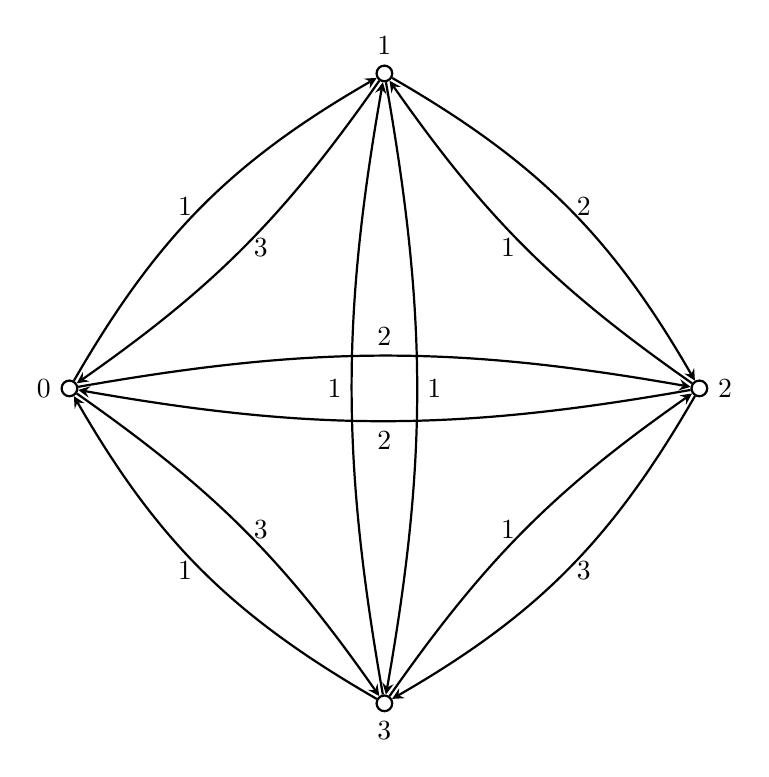
\begin{tikzpicture}
[nodedecorate/.style={shape=circle,inner sep=2pt,draw,thick},%
  arrowdecorate/.style={->,>=stealth,thick}]
% nodes or vertices
\node (0) at (-4,4) [nodedecorate] {};
\node [left] at (0.west) {$0$};
\node (1) at (0,8) [nodedecorate] {};
\node [above] at (1.north) {$1$};
\node (2) at (4,4) [nodedecorate] {};
\node [right] at (2.east) {$2$};
\node (3) at (0,0) [nodedecorate] {};
\node [below] at (3.south) {$3$};
% edges or lines
\path
(0) edge[arrowdecorate,bend left=15] node[left]{$1$} (1)
(0) edge[arrowdecorate,bend left=10] node[above]{$2$} (2)
(0) edge[arrowdecorate,bend left=10] node[right]{$3$} (3)
(1) edge[arrowdecorate,bend left=10] node[right]{$3$} (0)
(1) edge[arrowdecorate,bend left=15] node[right]{$2$} (2)
(1) edge[arrowdecorate,bend left=10] node[right]{$1$} (3)
(2) edge[arrowdecorate,bend left=10] node[below]{$2$} (0)
(2) edge[arrowdecorate,bend left=10] node[left]{$1$} (1)
(2) edge[arrowdecorate,bend left=15] node[right]{$3$} (3)
(3) edge[arrowdecorate,bend left=15] node[left]{$1$} (0)
(3) edge[arrowdecorate,bend left=10] node[left]{$1$} (1)
(3) edge[arrowdecorate,bend left=10] node[left]{$1$} (2);
\end{tikzpicture}
}
\subfigure[]{
\begin{tikzpicture}
[nodedecorate/.style={shape=circle,inner sep=2pt,draw,thick},%
  linedecorate/.style={-,thick}]
% nodes or vertices
\node (0) at (4,-4) [nodedecorate] {};
\node [right] at (0.east) {$0$};
\node (1) at (2,-2) [nodedecorate] {};
\node [right] at (1.east) {$1$};
\node (2) at (6,-6) [nodedecorate] {};
\node [right] at (2.east) {$2$};
\node (3) at (0,0) [nodedecorate] {};
\node [right] at (3.east) {$3$};
% edges or lines
\path
(3) edge[linedecorate] node[left]{$1$} (1)
(1) edge[linedecorate] node[left]{$1$} (0)
(0) edge[linedecorate] node[left]{$2$} (2);
\end{tikzpicture}
}
\caption{Prim's algorithm for digraphs. Above is the original digraph
  and below is the MST produced by Prim's algorithm.}
\label{fig:tree-forests:Prim_algorithm_digraph}
\end{figure}



\begin{center}
\fontsize{9pt}{9pt}
\selectfont
\tt
\begin{lstlisting}
        sage: A = matrix([[0,7,0,5,0,0,0],[0,0,8,9,7,0,0],[0,0,0,0,5,0,0],
         [0,0,0,0,15,6,0],[0,0,0,0,0,8,9],[0,0,0,0,0,0,11],[0,0,0,0,0,0,0]])
        sage: G = Graph(A, format = "adjacency_matrix", weighted = True)
        sage: E = G.edges(); E
        [(0, 1, 7), (0, 3, 5), (1, 2, 8), (1, 3, 9), (1, 4, 7), (2, 4, 5),
         (3, 4, 15), (3, 5, 6), (4, 5, 8), (4, 6, 9), (5, 6, 11)]
        sage: prim(G).edges()
        [(0, 1, 7), (0, 3, 5), (1, 2, 8), (1, 4, 7), (3, 5, 6), (4, 6, 9)]
\end{lstlisting}
\end{center}
%


\begin{figure}[!htbp]
\centering
\subfigure[]{
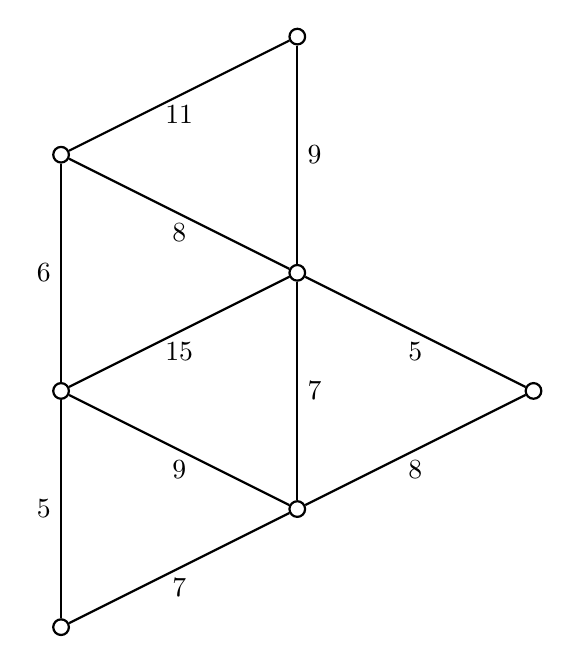
\begin{tikzpicture}
[nodedecorate/.style={shape=circle,inner sep=2pt,draw,thick},%
  linedecorate/.style={-,thick}]
% nodes or vertices
\node (0) at (0,0) [nodedecorate] {};
\node (1) at (3,1.5) [nodedecorate] {};
\node (2) at (6,3) [nodedecorate] {};
\node (3) at (0,3) [nodedecorate] {};
\node (4) at (3,4.5) [nodedecorate] {};
\node (5) at (0,6) [nodedecorate] {};
\node (6) at (3,7.5) [nodedecorate] {};
% edges or lines
\path
(0) edge[linedecorate] node[below]{$7$} (1)
(0) edge[linedecorate] node[left]{$5$} (3)
(1) edge[linedecorate] node[below]{$8$} (2)
(1) edge[linedecorate] node[below]{$9$} (3)
(1) edge[linedecorate] node[right]{$7$} (4)
(2) edge[linedecorate] node[below]{$5$} (4)
(3) edge[linedecorate] node[below]{$15$} (4)
(3) edge[linedecorate] node[left]{$6$} (5)
(4) edge[linedecorate] node[below]{$8$} (5)
(4) edge[linedecorate] node[right]{$9$} (6)
(5) edge[linedecorate] node[below]{$11$} (6);
\end{tikzpicture}
}
\subfigure[]{
\begin{tikzpicture}
[nodedecorate/.style={shape=circle,inner sep=2pt,draw,thick},%
  linedecorate/.style={-,thick}]
% nodes or vertices
\node (6) at (0,0) [nodedecorate] {};
\node [left] at (6.west) {$6$};
\node (4) at (2,2) [nodedecorate] {};
\node [left] at (4.west) {$4$};
\node (1) at (4,4) [nodedecorate] {};
\node [left] at (1.west) {$1$};
\node (2) at (6,2) [nodedecorate] {};
\node [left] at (2.west) {$2$};
\node (0) at (4,6) [nodedecorate] {};
\node [left] at (0.west) {$0$};
\node (3) at (4,8) [nodedecorate] {};
\node [left] at (3.west) {$3$};
\node (5) at (4,10) [nodedecorate] {};
\node [left] at (5.west) {$5$};
% edges or lines
\path
(6) edge[linedecorate] node[below]{$9$} (4)
(4) edge[linedecorate] node[below]{$7$} (1)
(1) edge[linedecorate] node[above]{$8$} (2)
(1) edge[linedecorate] node[right]{$7$} (0)
(0) edge[linedecorate] node[right]{$5$} (3)
(3) edge[linedecorate] node[right]{$6$} (5);
\end{tikzpicture}
}
\caption{Another example of Prim's algorithm. On the left is the
  original graph. On the right is the MST produced by Prim's algorithm.}
\label{fig:tree-forests:Prim_algorithm_digraph2}
\end{figure}


\subsection{Bor\r{u}vka's algorithm}

%%-----------------------------------------------------------------------%%
%%--- Binary trees ------------------------------------------------------%%

\section{Binary trees}

See section~3.3 of Gross and Yellen~\cite{GrossYellen1999}.

\begin{itemize}
\item binary codes

\item Huffman codes

\item Huffman algorithm
\end{itemize}


%%-----------------------------------------------------------------------%%
%%--- Tree traversals ---------------------------------------------------%%

\section{Tree traversals}

See section~3.5 of Gross and Yellen~\cite{GrossYellen1999}.

\begin{itemize}
\item stacks and queues

\item level-order traversal

\item pre-order traversal

\item post-order traversal

\item in-order traversal
\end{itemize}


%%-----------------------------------------------------------------------%%
%%--- Binary search trees -----------------------------------------------%%

\section{Binary search trees}

See section~3.6 of Gross and Yellen~\cite{GrossYellen1999}, and
chapter~12 of Cormen~et~al.~\cite{CormenEtAl2001}.

\begin{itemize}
\item records and keys

\item searching a binary search tree (BST)

\item inserting into a BST

\item deleting from a BST

\item traversing a BST

\item sorting using BST
\end{itemize}
